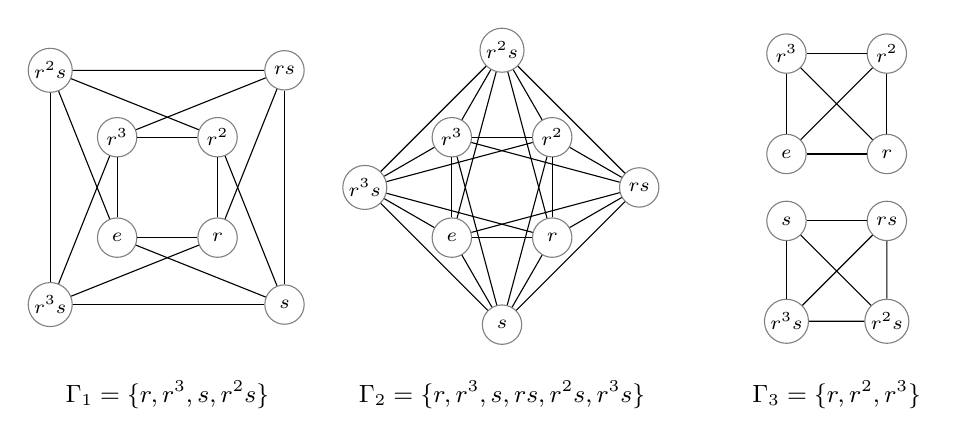
\begin{tikzpicture}[
    font=\footnotesize,
    scale=0.85,
    cell/.style = {font=\scriptsize, shape=circle, draw=gray, minimum width=0.5cm, inner sep=1pt}
    ]
    \begin{scope}
        \node[cell] (dih e)   at (0,   0)   {$e$};
        \node[cell] (dih r)   at (1.5, 0)   {$r$};
        \node[cell] (dih r2)  at (1.5, 1.5) {$r^2$};
        \node[cell] (dih r3)  at (0,   1.5) {$r^3$};
        \node[cell] (dih s)   at (2.5,  -1) {$s$};
        \node[cell] (dih rs)  at (2.5, 2.5) {$rs$};
        \node[cell] (dih r2s) at (-1,  2.5) {$r^2s$};
        \node[cell] (dih r3s) at (-1,  -1)  {$r^3s$};

        % Generating set: r, r3, s, r2s

        % Multiplication by r, r3
        \path [-] (dih e)  edge (dih r);
        \path [-] (dih r)  edge (dih r2);
        \path [-] (dih r2) edge (dih r3);
        \path [-] (dih r3) edge (dih e);

        \path [-] (dih s)   edge (dih rs);
        \path [-] (dih rs)  edge (dih r2s);
        \path [-] (dih r2s) edge (dih r3s);
        \path [-] (dih r3s) edge (dih s);

        % Multiplication by s, r2s
        \path [-] (dih e)  edge (dih s);
        \path [-] (dih e)  edge (dih r2s);
        \path [-] (dih r)  edge (dih rs);
        \path [-] (dih r)  edge (dih r3s);
        \path [-] (dih r2) edge (dih r2s);
        \path [-] (dih r2) edge (dih s);
        \path [-] (dih r3) edge (dih r3s);
        \path [-] (dih r3) edge (dih rs);

        % Set label
        \node[align=left, anchor=north, font=\small] at (0.75, -2) {$\Gamma_1 = \{r, r^3, s, r^2 s\}$};
    \end{scope}

    \begin{scope}[xshift=5cm]
        \node[cell] (dih3 e)   at (0,   0)   {$e$};
        \node[cell] (dih3 r)   at (1.5, 0)   {$r$};
        \node[cell] (dih3 r2)  at (1.5, 1.5) {$r^2$};
        \node[cell] (dih3 r3)  at (0,   1.5) {$r^3$};

        \node[cell] (dih3 s)   at (0.75, -1.3)  {$s$};
        \node[cell] (dih3 rs)  at (2.8, 0.75) {$rs$};
        \node[cell] (dih3 r2s) at (0.75, 2.8)    {$r^2s$};
        \node[cell] (dih3 r3s) at (-1.3, 0.75) {$r^3s$};

        % Generating set: r, r3, s, rs, r2s, r3s

        % Multiplication by r, r3
        \path [-] (dih3 e)  edge (dih3 r);
        \path [-] (dih3 r)  edge (dih3 r2);
        \path [-] (dih3 r2) edge (dih3 r3);
        \path [-] (dih3 r3) edge (dih3 e);
        \path [-] (dih3 s)   edge (dih3 rs);
        \path [-] (dih3 rs)  edge (dih3 r2s);
        \path [-] (dih3 r2s) edge (dih3 r3s);
        \path [-] (dih3 r3s) edge (dih3 s);

        % Multiplication by s, r2s
        \path [-] (dih3 e)  edge (dih3 s);
        \path [-] (dih3 e)  edge (dih3 r2s);
        \path [-] (dih3 r)  edge (dih3 rs);
        \path [-] (dih3 r)  edge (dih3 r3s);
        \path [-] (dih3 r2) edge (dih3 r2s);
        \path [-] (dih3 r2) edge (dih3 s);
        \path [-] (dih3 r3) edge (dih3 r3s);
        \path [-] (dih3 r3) edge (dih3 rs);

        % Multiplication by rs, r3s
        \path [-] (dih3 e)  edge (dih3 rs);
        \path [-] (dih3 e)  edge (dih3 r3s);
        \path [-] (dih3 r)  edge (dih3 r2s);
        \path [-] (dih3 r)  edge (dih3 s);
        \path [-] (dih3 r2) edge (dih3 r3s);
        \path [-] (dih3 r2) edge (dih3 rs);
        \path [-] (dih3 r3) edge (dih3 s);
        \path [-] (dih3 r3) edge (dih3 r2s);

        % Set label
        \node[align=left, anchor=north, font=\small] at (0.75, -2) {$\Gamma_2 = \{r, r^3, s, rs, r^2 s, r^3 s\}$};
    \end{scope}

    \begin{scope}[xshift=10cm, yshift=1.25cm]
        \node[cell] (dih2 e)   at (0,   0)   {$e$};
        \node[cell] (dih2 r)   at (1.5, 0)   {$r$};
        \node[cell] (dih2 r2)  at (1.5, 1.5) {$r^2$};
        \node[cell] (dih2 r3)  at (0,   1.5) {$r^3$};
        \node[cell] (dih2 s)   at (0,   -1)  {$s$};
        \node[cell] (dih2 rs)  at (1.5, -1)  {$rs$};
        \node[cell] (dih2 r2s) at (1.5, -2.5) {$r^2s$};
        \node[cell] (dih2 r3s) at (0,   -2.5) {$r^3s$};

        % Generating set: r, r2, r3

        % Multiplication by r, r3
        \path [-] (dih2 e)   edge (dih2 r);
        \path [-] (dih2 r)   edge (dih2 r2);
        \path [-] (dih2 r2)  edge (dih2 r3);
        \path [-] (dih2 r3)  edge (dih2 e);
        \path [-] (dih2 s)   edge (dih2 rs);
        \path [-] (dih2 rs)  edge (dih2 r2s);
        \path [-] (dih2 r2s) edge (dih2 r3s);
        \path [-] (dih2 r3s) edge (dih2 s);

        % Multiplication by r2
        \path [-] (dih2 e)   edge (dih2 r2);
        \path [-] (dih2 r)   edge (dih2 r3);
        \path [-] (dih2 s)   edge (dih2 r2s);
        \path [-] (dih2 rs)  edge (dih2 r3s);

        % Set label
        \node[align=left, anchor=north, font=\small] at (0.75, -3.25) {$\Gamma_3 = \{r, r^2, r^3\}$};
    \end{scope}


\end{tikzpicture}

